\documentclass{beamer}
\usepackage{graphicx}
\usepackage{xcolor}
\usepackage{tikz}
\usepackage{amsmath}

\definecolor{purpleblue}{RGB}{80, 80, 180}
\definecolor{novelPurple}{RGB}{98, 54, 255}
\definecolor{softPurple}{RGB}{180, 170, 255}
\definecolor{softGray}{RGB}{235, 235, 245}
\definecolor{lightText}{RGB}{90, 90, 110}

\usetheme{Madrid}
\usecolortheme{dolphin}
\graphicspath{{static/course_materials/}{static/hard/}{./}}

\setbeamerfont{title}{size=\Large,series=\bfseries}
\setbeamerfont{frametitle}{size=\LARGE,series=\bfseries}
\setbeamercolor{frametitle}{fg=white, bg=novelPurple}
\setbeamercolor{title}{fg=white, bg=purpleblue}

\title[SAT Hard Question 15]{\textbf{SAT Hard Question\\ Set 15}}
\author{\textbf{Jack Zeng}}
\institute{\textcolor{white}{\textbf{Novel Prep}}}
\date{\today}

\begin{document}

\begin{frame}
    \titlepage
    \vfill
    \begin{flushright}
        \textcolor{purpleblue}{\Huge \textbf{Novel Prep}}
    \end{flushright}
\end{frame}

\begin{frame}
    \begin{tikzpicture}[remember picture, overlay]
        \shade[top color=softPurple, bottom color=softGray]
            (current page.north west) rectangle (current page.south east);
        \node[align=center] at (current page.center) {
            {\Huge\bfseries\textcolor{purpleblue}{Novel Prep}} \\[0.5cm]
            {\Large\itshape\textcolor{lightText}{Phase 2 · Hard Question Practice}}
        };
    \end{tikzpicture}
\end{frame}

\begin{frame}{Overview}
    \tableofcontents
\end{frame}

\begin{frame}
\section{Hard Question Set 15}
    \begin{tikzpicture}[remember picture, overlay]
        \shade[top color=softPurple, bottom color=softGray]
            (current page.north west) rectangle (current page.south east);
        \node[align=center] at (current page.center) {
            {\LARGE\bfseries\textcolor{purpleblue}{Hard Question Set 15}} \\[0.5cm]
            {\Large\itshape\textcolor{lightText}{25 SAT-style challenge problems}}
        };
    \end{tikzpicture}
\end{frame}

% --- Question 1 ---
\begin{frame}{Question 1}
\small
For the function
\[
f(x) = a\sqrt{b - x} + \frac{12}{\sqrt{b - x}},
\]
\(a\) and \(b\) are constants, and \(f(4) = 0\). If \(f(5) > 0\), which of the following could be a value for \(a + b\)?
\vspace{0.35cm}
\begin{enumerate}
    \item[A.] \(-20\)
    \item[B.] \(-12\)
    \item[C.] \(-8\)
    \item[D.] \(-4\)
\end{enumerate}
\end{frame}
\begin{frame}{Answer 1}
\small
\textbf{Correct Answer:} D
\end{frame}

% --- Question 2 ---
\begin{frame}{Question 2}
\small
\[
\frac{16}{a} = \frac{16}{b} + \frac{16}{c}
\]
Which of the following expresses \(a\) in terms of \(b\) and \(c\)?
\vspace{0.35cm}
\begin{enumerate}
    \item[A.] \(a = \dfrac{b + c}{bc}\)
    \item[B.] \(a = \dfrac{bc}{b + c}\)
    \item[C.] \(a = bc(b + c)\)
    \item[D.] \(a = 16bc(b + c)\)
\end{enumerate}
\end{frame}
\begin{frame}{Answer 2}
\small
\textbf{Correct Answer:} B
\end{frame}

% --- Question 3 ---
\begin{frame}{Question 3}
\small
\[
\frac{ax^3 + bx^2 + cx + d}{(x^2 - 9)(x + 2)} = \frac{5}{x + 3} + \frac{6x}{x - 3}
\]
What is the value of \(a + b + c\)?
\end{frame}
\begin{frame}{Answer 3}
\small
\textbf{Final Answer:} $\boxed{72}$
\end{frame}

% --- Question 4 ---
\begin{frame}{Question 4}
\small
There are two lawn mowing companies. Company A charges a flat fee of \(\$80\) for the first hour, then an hourly rate of \(\$60\) for each additional hour. Company B charges no flat fee, but an hourly rate of \(\$75\) per hour. After how many minutes will company B's total cost exceed company A's?
\end{frame}
\begin{frame}{Answer 4}
\small
\textbf{Final Answer:} $\boxed{80}$
\end{frame}

% --- Question 5 ---
\begin{frame}{Question 5}
\small
\[
\begin{aligned}
\frac{5}{6}x + ay &= b \\
\frac{11}{10}x + cy &= 2d
\end{aligned}
\]
If the system of equations above has infinitely many solutions, what must be the value of \(\dfrac{b}{d}\)?
\end{frame}
\begin{frame}{Answer 5}
\small
\textbf{Final Answer:} $\boxed{\dfrac{50}{33}}$
\end{frame}

% --- Question 6 ---
\begin{frame}{Question 6}
\small
\(a\) is \(540\%\) more than \(b\) and \(b\) is \(0.02\%\) of \(c\). If \(a\) is \(k\%\) of \(c\), then what must \(k\) equal?
\end{frame}
\begin{frame}{Answer 6}
\small
\textbf{Final Answer:} $\boxed{0.128}$
\end{frame}

% --- Question 7 ---
\begin{frame}{Question 7}
\small
\[
f(t) = a \cdot 2^{\frac{2t}{11}}
\]
The given function \(f(t)\) models the amount of money in an investment account \(t\) years after the account is opened, where \(a\) is a constant. How many months will it take for the initial investment to increase by \(700\%\)?
\end{frame}
\begin{frame}{Answer 7}
\small
\textbf{Final Answer:} $\boxed{198}$
\end{frame}

% --- Question 8 ---
\begin{frame}{Question 8}
\small
The function \(f\) is defined by
\[
f(x) = k^{3kx} + b
\]
for \(x \ge 0\). \(k\) and \(b\) are positive constants and \(k < 1\). Which of the following must be true?

\begin{itemize}
\item I. The maximum value of the function is displayed as a constant or coefficient of the function.
\item II. \(f(1) = f(0) \cdot k\)
\item III. \(f(a) < b\) for some \(a > 0\)
\end{itemize}
\vspace{0.35cm}
\begin{enumerate}
    \item[A.] I only
    \item[B.] II and III only
    \item[C.] I and III only
    \item[D.] Neither I, II, nor III
\end{enumerate}
\end{frame}
\begin{frame}{Answer 8}
\small
\textbf{Correct Answer:} D
\end{frame}

% --- Question 9 ---
\begin{frame}{Question 9}
\small
\[
15x^{18} + kx^{9} + 24
\]
The expression above has factors \(ax^{9} + b\) and \(cx^{9} + d\), where \(a\), \(b\), \(c\), and \(d\) are all integer constants. What is the maximum value of \(k\)?
\end{frame}
\begin{frame}{Answer 9}
\small
\textbf{Final Answer:} $\boxed{361}$
\end{frame}

% --- Question 10 ---
\begin{frame}{Question 10}
\small
\[
(hx + k)(qx + z) = ax^{2} + bx + 35
\]
For the expression above, \(h\), \(k\), \(q\), and \(z\) are all integer constants. Which of the following must be an integer?

\begin{itemize}
\item I. \(\dfrac{35}{k}\)
\item II. \(b\)
\item III. \(-\dfrac{a}{q}\)
\end{itemize}
\vspace{0.35cm}
\begin{enumerate}
    \item[A.] I and II only
    \item[B.] II and III only
    \item[C.] I and III only
    \item[D.] I, II, and III
\end{enumerate}
\end{frame}
\begin{frame}{Answer 10}
\small
\textbf{Correct Answer:} D
\end{frame}

% --- Question 11 ---
\begin{frame}{Question 11}
\small
\[
f(x) = -3x^{2} + bx + c
\]
In the given quadratic function, \(b\) and \(c\) are constants. The graph of \(y = f(x)\) in the \(xy\)-plane is a parabola that has a vertex at the point \((h, k)\), where \(h\) and \(k\) are constants. If \(f(-4) = f(8)\), and the quadratic function has \(x\)-intercepts at \((r, 0)\) and \((s, 0)\), which of the following must be true?

\begin{itemize}
\item I. \(r + s = 4\)
\item II. \(b < 0\)
\item III. \(c < k\)
\end{itemize}
\vspace{0.35cm}
\begin{enumerate}
    \item[A.] I and II only
    \item[B.] II and III only
    \item[C.] I and III only
    \item[D.] I, II, and III
\end{enumerate}
\end{frame}
\begin{frame}{Answer 11}
\small
\textbf{Correct Answer:} C
\end{frame}

% --- Question 12 ---
\begin{frame}{Question 12}
\small
A quadratic function models a rock's height, in feet, above the ground in terms of the time, in seconds, after it is thrown. The rock was thrown from an initial height of \(c\) feet above the ground and reached a maximum height of \(200\) feet above the ground \(3\) seconds after it was thrown. Then it hit the ground \(8\) seconds after being thrown. At what initial height \(c\) was the rock thrown?
\end{frame}
\begin{frame}{Answer 12}
\small
\textbf{Final Answer:} $\boxed{128}$
\end{frame}

% --- Question 13 ---
\begin{frame}{Question 13}
\small
\[
2rx^{2} - 5sx + 8r = 0
\]
If the quadratic equation above has one real solution and \(rs = 160\), what is \(\lvert r + s \rvert\)?
\end{frame}
\begin{frame}{Answer 13}
\small
\textbf{Final Answer:} $\boxed{26}$
\end{frame}

% --- Question 14 ---
\begin{frame}{Question 14}
\small
\[
f(x) = -(x + a)^{2}(x - b)(x - c)
\]
For the polynomial function above, \(a\), \(b\), and \(c\) are positive constants. Let \(b < k < c\) for some constant \(k\). Which of the following must be true?

\begin{itemize}
\item I. \(k > 0\)
\item II. \(f(k) > 0\)
\item III. \(f(0) > 0\)
\end{itemize}
\vspace{0.35cm}
\begin{enumerate}
    \item[A.] I and II only
    \item[B.] II and III only
    \item[C.] I and III only
    \item[D.] I, II, and III
\end{enumerate}
\end{frame}
\begin{frame}{Answer 14}
\small
\textbf{Correct Answer:} A
\end{frame}

% --- Question 15 ---
\begin{frame}{Question 15}
\small
Three consecutive even integers are ordered from smallest to largest. \(5\) times the first integer is at least \(9\) more than the sum of the second and third integers. What is the minimum possible value for the second integer?
\end{frame}
\begin{frame}{Answer 15}
\small
\textbf{Final Answer:} $\boxed{8}$
\end{frame}

% --- Question 16 ---
\begin{frame}{Question 16}
\small
If a car accelerates at \(108\) kilometers per hour squared, what is its acceleration in meters per minute squared? (\(1\) kilometer \(= 1000\) meters)
\end{frame}
\begin{frame}{Answer 16}
\small
\textbf{Final Answer:} $\boxed{30}$
\end{frame}

% --- Question 17 ---
\begin{frame}{Question 17}
\small
In triangle \(\triangle ABC\), the measure of \(\angle B\) is \(90^\circ\), \(AB\) is a leg with a length of \(12\), and point \(D\) lies on segment \(AC\). Which of the following must be true?

\begin{itemize}
\item I. \(BC = 12\tan(\angle CAB)\)
\item II. \(\cos(\angle ABD) - \sin(\angle DBC) = 0\)
\item III. \(\angle ABD = \angle BDC\)
\end{itemize}
\vspace{0.35cm}
\begin{enumerate}
    \item[A.] I and II only
    \item[B.] II and III only
    \item[C.] I and III only
    \item[D.] I, II, and III
\end{enumerate}
\end{frame}
\begin{frame}{Answer 17}
\small
\textbf{Correct Answer:} A
\end{frame}

% --- Question 18 ---
\begin{frame}{Question 18}
\small
In triangle \(\triangle ABC\), the measure of \(\angle B\) is \(90^\circ\), and \(BD\) is an altitude of the triangle. The length of \(BC\) is \(10\) and \(\angle ABD = 60^\circ\). What is the length of \(AD\)?
\end{frame}
\begin{frame}{Answer 18}
\small
\textbf{Final Answer:} $\boxed{15}$
\end{frame}

% --- Question 19 ---
\begin{frame}{Question 19}
\small
In the circle above, \(AC\) is a diameter and \(\angle ACB = 20^\circ\). If the circumference of the circle is \(90\) inches, what is the length of arc \(BC\)?

\begin{center}
    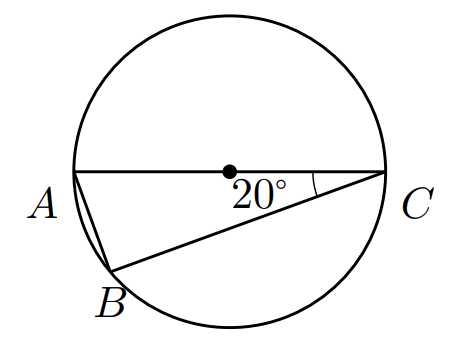
\includegraphics[width=0.42\linewidth]{hard_15_f19.png}
\end{center}
\end{frame}
\begin{frame}{Answer 19}
\small
\textbf{Final Answer:} $\boxed{35}$
\end{frame}

% --- Question 20 ---
\begin{frame}{Question 20}
\small
In the \(xy\)-plane, the graph of \(x^{2} + 6x + y^{2} + 2y = 15\) is a circle. Line \(k\) has a slope of \(\dfrac{3}{4}\) and is tangent to this circle at the point \((a, b)\), where \(b\) is negative. What is the value of \(b\)?
\end{frame}
\begin{frame}{Answer 20}
\small
\textbf{Final Answer:} $\boxed{-5}$
\end{frame}

% --- Question 21 ---
\begin{frame}{Question 21}
\small
Rectangular prism \(A\) and rectangular prism \(B\) are similar. The height of rectangular prism \(A\) is \(4\) inches and the height of rectangular prism \(B\) is \(10\) inches. If the volume of prism \(A\) is \(200\) cubic inches, then what is the volume of prism \(B\)?
\end{frame}
\begin{frame}{Answer 21}
\small
\textbf{Final Answer:} $\boxed{3125}$
\end{frame}

% --- Question 22 ---
\begin{frame}{Question 22}
\small
Consider a square right pyramid with a volume of \(400\) cubic inches and a slant height of \(13\) inches. The pyramid's length, width, and height (in inches) are all integers. What is the surface area of the pyramid in square inches?
\end{frame}
\begin{frame}{Answer 22}
\small
\textbf{Final Answer:} $\boxed{360}$
\end{frame}

% --- Question 23 ---
\begin{frame}{Question 23}
\small
Data set \(A\) consists of \(4\) integers greater than or equal to \(10\) but less than or equal to \(20\). Data set \(B\) consists of the same four integers and adds one more integer, which must also be between \(10\) and \(20\). What is the largest possible difference between the mean of data set \(A\) and the mean of data set \(B\)?
\end{frame}
\begin{frame}{Answer 23}
\small
\textbf{Final Answer:} $\boxed{2}$
\end{frame}

% --- Question 24 ---
\begin{frame}{Question 24}
\small
\begin{center}
\begin{tabular}{|c|c|}
\hline
Data & Frequency \\
\hline
1 & 2 \\
2 & 5 \\
3 & 6 \\
4 & 5 \\
5 & 2 \\
\hline
\end{tabular}
\end{center}

The frequency table above summarizes data set \(A\). Data set \(B\) is created by multiplying all of the values in data set \(A\) by \(2\). Which of the following must be true?

\begin{itemize}
\item I. The difference between the mean and median of data set \(B\) is \(0\).
\item II. The standard deviation of data set \(B\) is equal to the standard deviation of data set \(A\).
\item III. The range of data set \(B\) is double the range of data set \(A\).
\end{itemize}
\vspace{0.35cm}
\begin{enumerate}
    \item[A.] I and II only
    \item[B.] II and III only
    \item[C.] I and III only
    \item[D.] I, II, and III
\end{enumerate}
\end{frame}
\begin{frame}{Answer 24}
\small
\textbf{Correct Answer:} C
\end{frame}

% --- Question 25 ---
\begin{frame}{Question 25}
\small
A sample of students was selected at random from all 11th graders at a school. Based on the sample, it is estimated that the proportion of 11th graders in at least one AP class is \(60\%\) with a margin of error of \(5\%\). Which of the following conclusions are appropriate?

\begin{itemize}
\item I. It is not possible for just \(40\%\) of the 11th graders in the school to be in at least one AP class.
\item II. It is plausible that the proportion of all students at the school in at least one AP class is between \(45\%\) and \(55\%\).
\item III. If the sample size is increased, the margin of error will drop below \(5\%\).
\end{itemize}
\vspace{0.35cm}
\begin{enumerate}
    \item[A.] I and II only
    \item[B.] II and III only
    \item[C.] III only
    \item[D.] I, II, and III
\end{enumerate}
\end{frame}
\begin{frame}{Answer 25}
\small
\textbf{Correct Answer:} C
\end{frame}

\begin{frame}{}
    \begin{tikzpicture}[remember picture, overlay]
        \shade[top color=novelPurple!40, bottom color=white]
            (current page.north west) rectangle (current page.south east);
        \fill[white, opacity=0.15] (current page.center) circle (5cm);
        \foreach \x in {1,2,3,4,5} {
            \fill[novelPurple, opacity=0.12] (rand*10-5, rand*7-3.5) circle (0.1+\x*0.05);
        }
    \end{tikzpicture}
    \centering
    \vspace{5em}
    {\Huge \textbf{\textcolor{novelPurple}{Thank You!}}} \\[1em]
    {\large \textcolor{gray}{We appreciate your time and focus.}} \\[3em]
    {\LARGE \textbf{\textcolor{novelPurple}{\textsf{Novel Prep}}}}
    \vfill
\end{frame}

\end{document}
